\subsection{Robotic setup}
\textit{James} is an \textit{upper-torso humanoid robot} with the size of an 
about ten years old boy, a total weight of about 8 kilograms and 22 degrees 
of freedom (DOF) \cite{JHRAUW06-12}. James consists of a head on a special 
neck , a left arm with a peculiar shoulder and the torso.

\begin{figure}
\centering
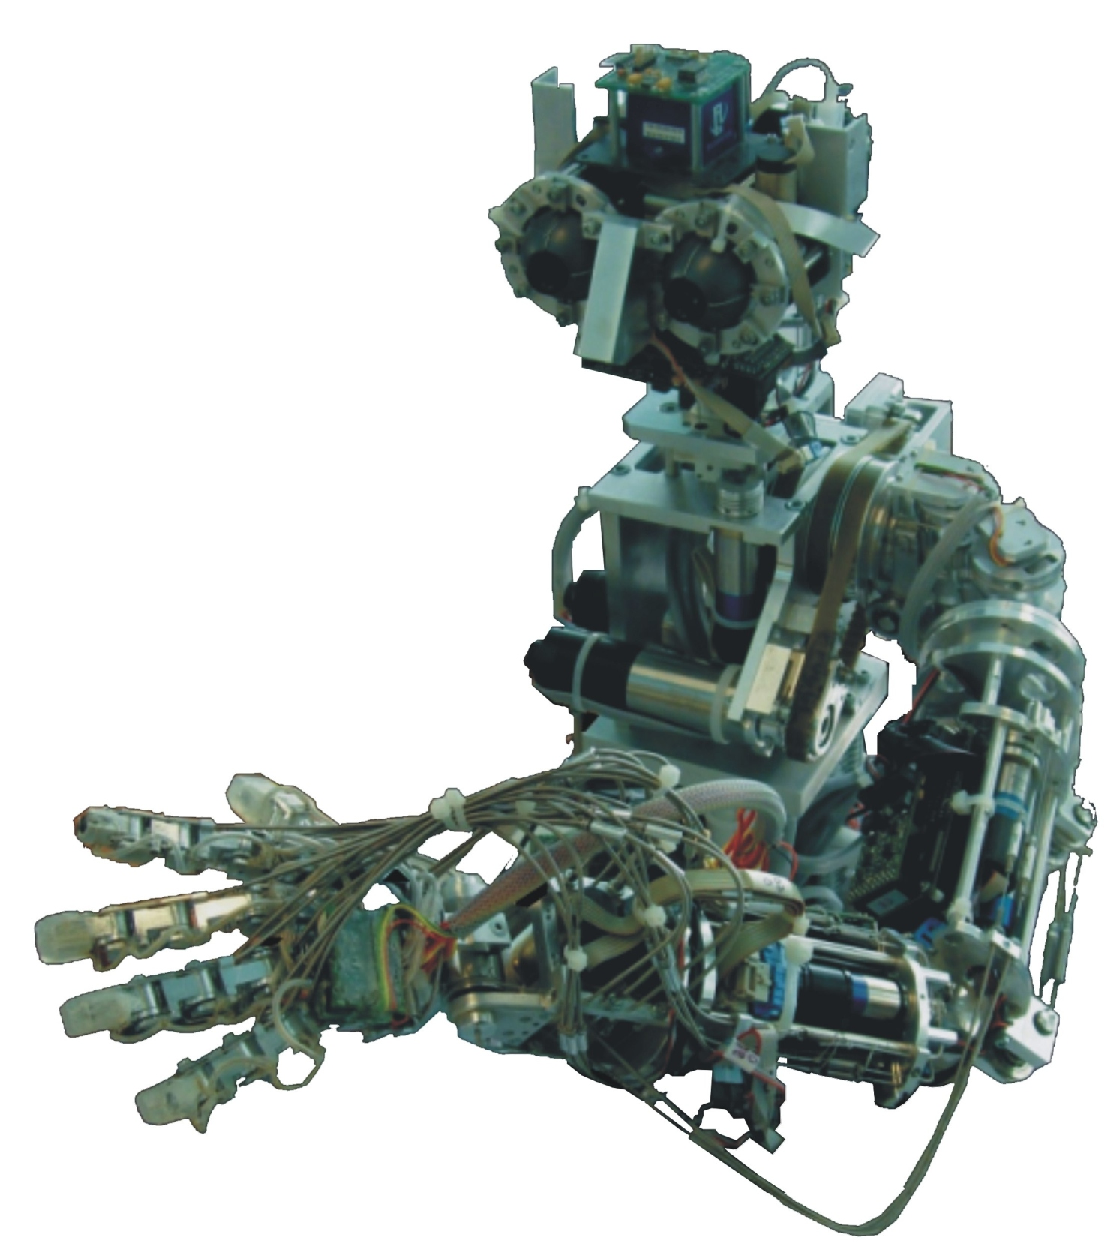
\includegraphics[width=2in]{imgs/james.ps}
\caption{James}
\label{figJames}
\end{figure}
